
\section{Introduction}
With the great development of modern cities, the rapid growth of population and the acceleration of urbanization has made transportation systems to an essential infrastructure. In the meantime, transportation systems are becoming more and more complex, which causes great pressure on urban traffic management. As a result, it is important to develop the Intelligent Transportation System (ITS)\cite{ITS} for efficient traffic management.

Modern transportation systems contain road vehicles, railway transportation and a variety of newly emerged shared travel modes, including online ride-hailing, bike-sharing, etc. In order to alleviate transportation related problems and manage the expanding transportation systems efficiently, traffic prediction or traffic forecasting is brought up for ITS by researchers in recent years. Traffic prediction is the process of analyzing urban road traffic conditions, including flow, speed and density, mining traffic patterns, and predicting road traffic trends. Traffic prediction can not only provide a scientific basis for traffic managers to perceive traffic congestion and limit vehicles in advance, but also provide a guarantee for travelers to choose proper travel routes and improve travel efficiency.

Traffic prediction is typically based on the consideration of historical traffic state data. In the development of intelligent transportation systems, traffic states are detected by traffic sensors, bus and metro transactions logs, traffic surveillance cameras and GPS devices. However, traffic state data is hard to manage because it involves large data volumes with high dimensionality. Its typical characteristic is that it contains both spatial and temporal domains.
% The traffic state in a specific location has both spatial dependency, which may not be affected only by nearby areas, and temporal dependency, which may be periodic.
Therefore, traffic prediction becomes a challenging topic because of spatial and temporal dependencies.
\begin{enumerate}
    \item \textbf{Spatial dependency.} Urban road network has a topological structure that seriously affects the change of traffic state of each road. To be specific, the upstream traffic state influences the downstream roads for the reason like vehicle transfer.
    
    \item \textbf{Temporal dependency.} Traffic state varies over time with periodicity. For example, in general, the traffic state over weekdays are similar to each other but has a huge difference with holidays, and vice versa. In detail, the traffic state at a specific moment is impacted by the previous moments or even hours.
\end{enumerate}

Traditional time series prediction models (e.g., Moving Average (MA), Auto-regressive (AR), Auto-regressive Integrated Moving Average (ARIMA)) cannot handle such spatiotemporal prediction scenarios well. Therefore, to address the complex dependencies, deep learning methods have been introduced to this area.

Graph convolution networks (GCN)\cite{GCN0} becomes popular in recent years due to its ability to capture spatiotemporal dependencies efficiently. Many GCN-based models reached state-of-the-art performance, such as STGCN\cite{STGCN}, DCRNN\cite{DCRNN}, Graph WaveNet\cite{GWNET} and AGCRN\cite{AGCRN}. To represent road network, a graph is constructed where each node in the graph stands for a road segment or a traffic sensor. And edges means connectivity between road segments or sensors. As a result, spatial dependency can be extracted directly from the graph. Concerning temporal dependency, every node is linked with a feature vector that consists of traffic states at each moment. Several methods were applied such as recurrent neural networks (RNN) and 1D convolutions. As mentioned above, in GCN-based models, spatial dependency is expressed only by the static relationship among roads in the graph. However, the traffic condition in real world is much more complicated. For example, the main roads in a city are often congested during peak hours. Although it is usually the shortest path to travel through main roads, commuters will probably prefer a father but clearer path. That is, the graph only shows the road connectivity which cannot represent the transfer preference by real drivers. Despite that it is impractical to collect all the traffic patterns, the trajectories reflect them well and thoroughly. In addition, when counting road flow or calculating road traffic speed, a trajectory is treated as discrete points, while the road transfer information naturally lies in the sequential order of the trajectory. Fortunately, such trajectories can be tracked by GPS devices and mobile apps with GPS service, and we have a completely raw GPS dataset which is copied directly from the logs of GPS devices in the taxis of Shenzhen.

\begin{figure}[htb]
    \centering
    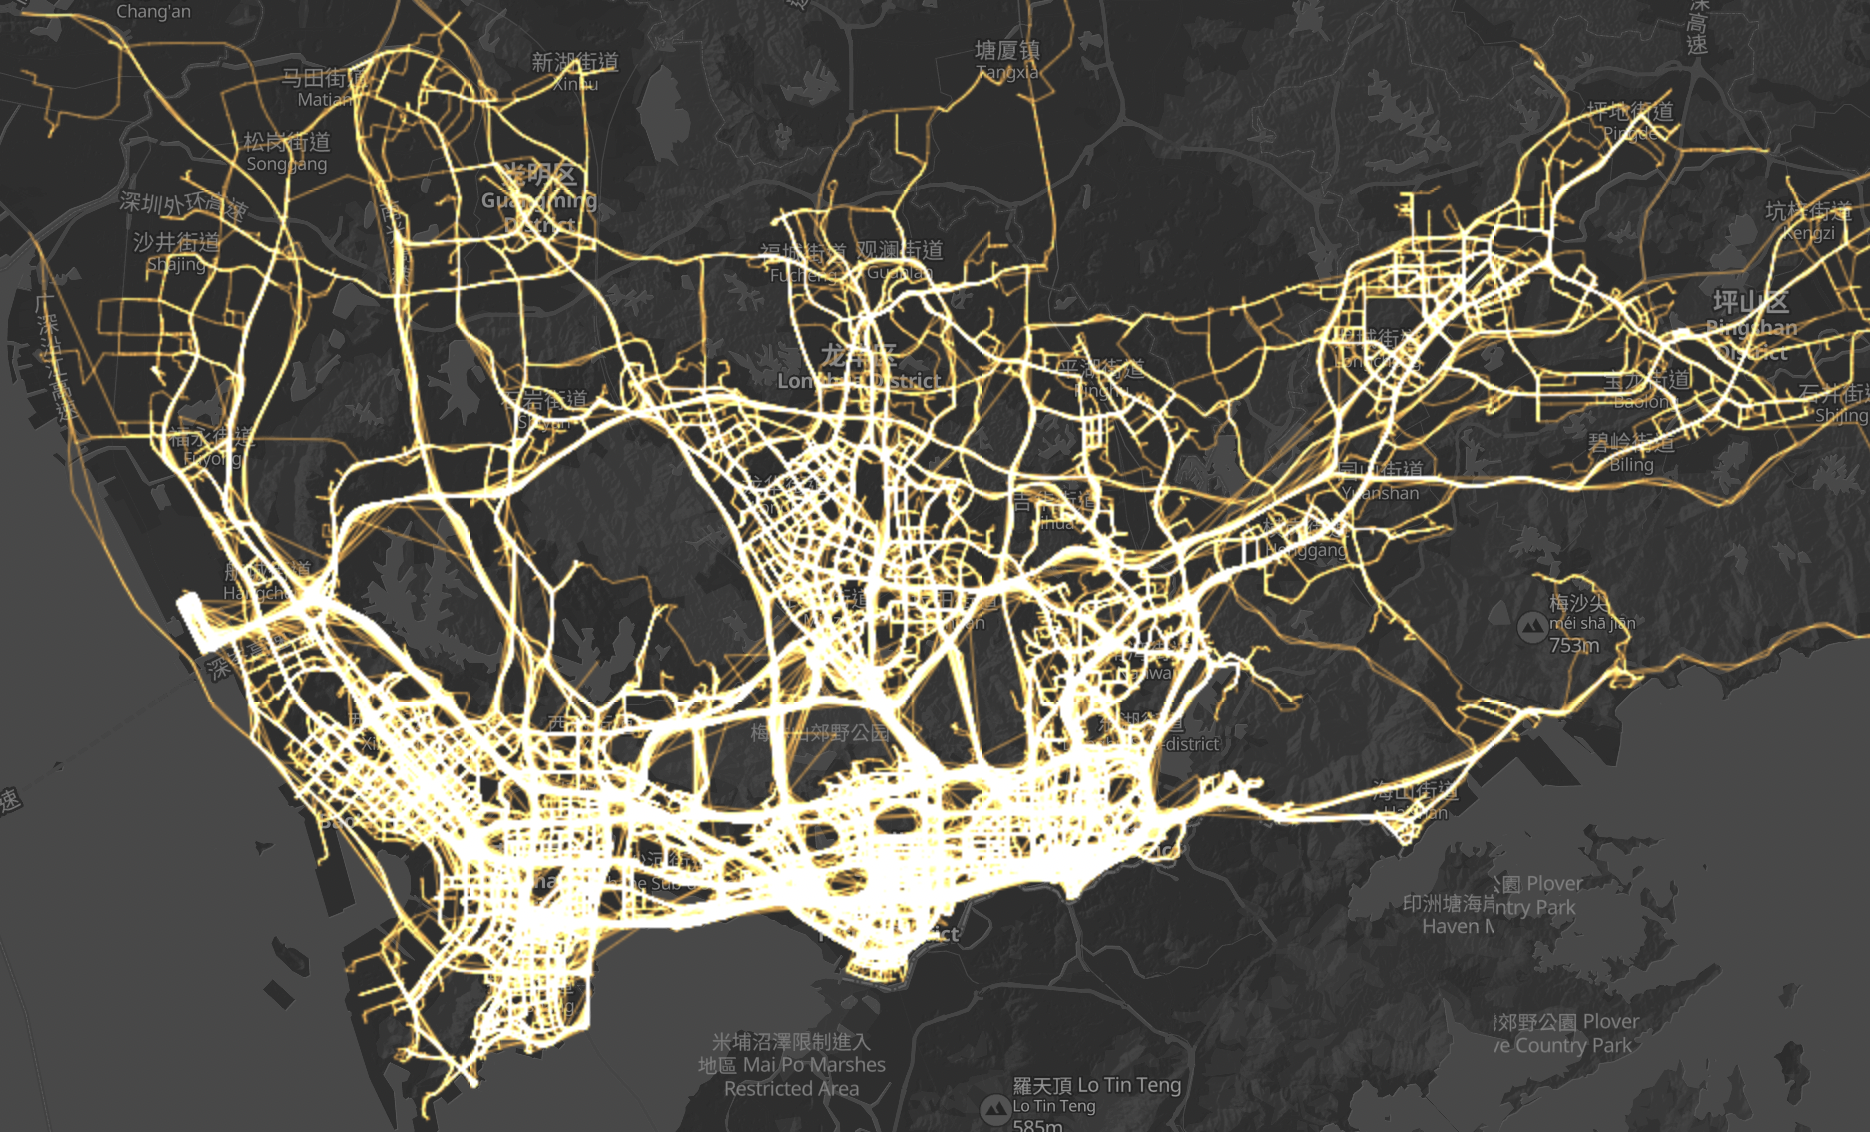
\includegraphics[width=\textwidth]{images/traj_map.png}
    \caption{Shenzhen taxi trajectories heatmap.}
    \label{fig: traj_map}
  \end{figure}

Based on these facts, we believe that the trajectories will give us the actual road transfer information. By analyzing road transfer, we propose a concept named \textit{trajectory-based road correlation} that stands for the relevance or similarity among roads. With this, a better spatial dependency can be captured. Therefore, the focus of this paper is to design a general method to extract road correlation through trajectories and utilize it for state-of-the-art neural networks to predict traffic state.

To summarize, in this paper, we propose a procedure to learn \textit{trajectory-based road correlation} via GPS data and use it to improve traffic state prediction.

The contribution of our paper is:
\begin{itemize}
    \item We build a road-network-based trajectory dataset upon completely raw GPS data.
    \item We propose a procedure to learn road correlation through trajectories.
    \item We improve traffic state prediction by utilizing the \textit{trajectory-based road correlation}.
\end{itemize}
